\documentclass[border = 120pt]{standalone}

\usepackage[landscape]{geometry}
\usepackage{tikz}
\usetikzlibrary{mindmap}
\usepackage{metalogo}
\usepackage{dtklogos}
\begin{document}
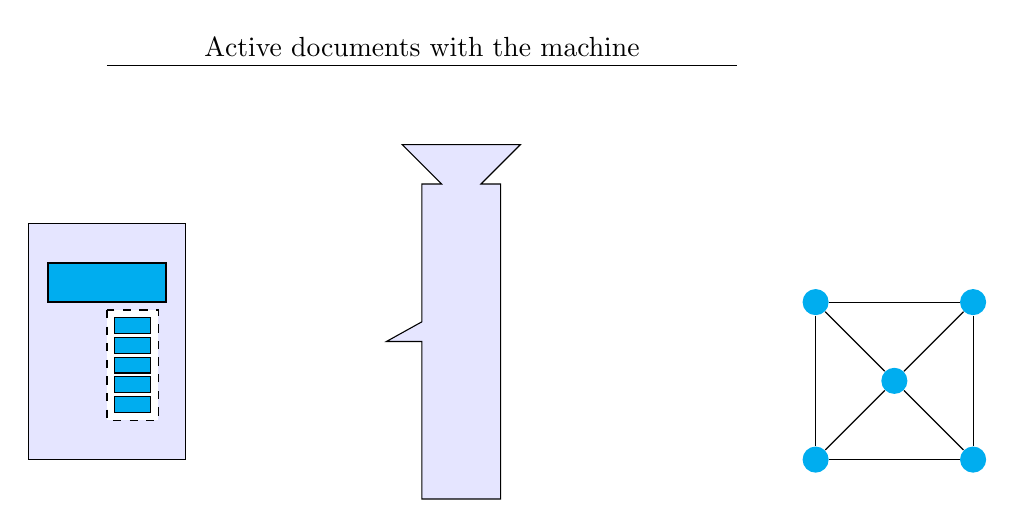
\begin{tikzpicture}

\draw[-] (-9,5) -- (-1,5) node[pos=.5,sloped,above] {Active documents with the machine};

%Mother Ship
\draw[fill=blue!10] (-8,0) rectangle (-10, 3);
\draw[style=thick, fill=cyan] (-9.75, 2) rectangle (-8.25, 2.5);

%Jupyter Box
\draw[style=dashed, fill=white] (-9, 1.9) rectangle (-8.35, 0.5);
\draw[fill=cyan] (-8.9, 1.8) rectangle (-8.45, 1.6);
\draw[fill=cyan] (-8.9, 1.55) rectangle (-8.45, 1.35);
\draw[fill=cyan] (-8.9, 1.3) rectangle (-8.45, 1.1);
\draw[fill=cyan] (-8.9, 1.05) rectangle (-8.45, 0.85);
\draw[fill=cyan] (-8.9, 0.8) rectangle (-8.45, 0.6);

% First machine
\path[draw, fill=blue!10] (-5, -0.5) -- (-5, 1.5) -- (-5.45, 1.5) -- (-5, 1.75) -- (-5, 3.5) -- (-4.75, 3.5) -- (-5.25, 4) -- (-3.75, 4) --(-4.25, 3.5) -- (-4, 3.5) -- (-4, -0.5) -- cycle;

// Nodes
\tikzstyle{every node} = [circle]
\node[fill=cyan] (a) at (0, 0) { };
\node[fill=cyan] (b) at (2, 0) { };
\node[fill=cyan] (c) at (2, 2) { };
\node[fill=cyan] (d) at (0, 2) { };
\node[fill=cyan] (e) at (1, 1) { };
\foreach \from/\to in {a/b, b/c, c/d, a/d, a/e, e/b, c/e, d/e}
\draw [-] (\from) -- (\to);

\end{tikzpicture}
\end{document}















